\documentclass[12pt,a4paper]{article}
\usepackage[utf8]{inputenc}
\usepackage[T1]{fontenc}
\usepackage{amsmath,amssymb}
\usepackage{pgfplots}
\usepackage{tikz}
\usepackage{lmodern}
\usepackage{graphicx}
\usepackage{hyperref}
\usepackage{listings}
\usepackage{xcolor}
\usepackage{enumitem}
\usepackage{fancyhdr}
\usepackage{lastpage}
\usepackage[left=2.5cm,right=2.5cm,top=2.5cm,bottom=2.5cm]{geometry}
\usepackage[table]{xcolor}
\usepackage{array}
\usepackage{hyperref}
\usepackage{nameref}

\pagestyle{fancy}
\fancyhf{}
\renewcommand{\headrulewidth}{0pt}
\rfoot{\thepage\ af \pageref{LastPage}}

\title{Forløbsplan}
\author{Anders S. Østergaard}
\date{\today}

\definecolor{codegreen}{rgb}{0,0.6,0}
\definecolor{codegray}{rgb}{0.5,0.5,0.5}
\definecolor{codepurple}{rgb}{0.58,0,0.82}
\definecolor{backcolour}{rgb}{0.95,0.95,0.92}
\definecolor{darkerlightblue}{rgb}{0.1, 0.3, 0.5}

\lstdefinestyle{mystyle}{
	backgroundcolor=\color{backcolour},   
	commentstyle=\color{codegreen},
	keywordstyle=\color{darkerlightblue},
	numberstyle=\tiny\color{codegray},
	stringstyle=\color{codepurple},
	basicstyle=\ttfamily\footnotesize,
	breakatwhitespace=false,         
	breaklines=true,                 
	captionpos=b,                    
	keepspaces=true,                 
	numbers=left,                    
	numbersep=5pt,                  
	showspaces=false,                
	showstringspaces=false,
	showtabs=false,                  
	tabsize=2
}
\lstset{style=mystyle}
\usepackage{matlab-prettifier}
\usepackage{listings}
\usepackage{color}

\definecolor{mygreen}{rgb}{0,0.6,0}
\definecolor{mygray}{rgb}{0.5,0.5,0.5}
\definecolor{mymauve}{rgb}{0.58,0,0.82}

\lstset{ 
	backgroundcolor=\color{white},   % choose the background color; you must add \usepackage{color} or \usepackage{xcolor}; should come as last argument
	basicstyle=\footnotesize,        % the size of the fonts that are used for the code
	breakatwhitespace=false,         % sets if automatic breaks should only happen at whitespace
	breaklines=true,                 % sets automatic line breaking
	captionpos=b,                    % sets the caption-position to bottom
	commentstyle=\color{mygreen},    % comment style
	deletekeywords={...},            % if you want to delete keywords from the given language
	escapeinside={\%*}{*)},          % if you want to add LaTeX within your code
	extendedchars=true,              % lets you use non-ASCII characters; for 8-bits encodings only, does not work with UTF-8
	firstnumber=1000,                % start line enumeration with line 1000
	frame=single,	                   % adds a frame around the code
	keepspaces=true,                 % keeps spaces in text, useful for keeping indentation of code (possibly needs columns=flexible)
	keywordstyle=\color{blue},       % keyword style
	language=Octave,                 % the language of the code
	morekeywords={*,...},            % if you want to add more keywords to the set
	%numbers=left,                    % where to put the line-numbers; possible values are (none, left, right)
	numbersep=5pt,                   % how far the line-numbers are from the code
	numberstyle=\tiny\color{mygray}, % the style that is used for the line-numbers
	rulecolor=\color{black},         % if not set, the frame-color may be changed on line-breaks within not-black text (e.g. comments (green here))
	showspaces=false,                % show spaces everywhere adding particular underscores; it overrides 'showstringspaces'
	showstringspaces=false,          % underline spaces within strings only
	showtabs=false,                  % show tabs within strings adding particular underscores
	stepnumber=2,                    % the step between two line-numbers. If it's 1, each line will be numbered
	stringstyle=\color{mymauve},     % string literal style
	tabsize=2,	                   % sets default tabsize to 2 spaces
	title=\lstname                   % show the filename of files included with \lstinputlisting; also try caption instead of title
}
\begin{document}
	\begin{titlepage}
	\centering
	\vspace*{6cm}
	{\Huge\bfseries SWROB2\par Exam\par}
	\vspace{2cm}
	Submitted by: \par 
	\begin{table}[!h]
		\centering
		\begin{tabular}{|l|l|l|}
			\hline
			Study nr  & Name 					   & Study line\\\hline
			202005180 & Nicolaj Meldgaard Pedersen & E\\\hline
			202105443 & Johannes Baagøe 		   & E\\\hline
			201270449 & Anders Sandø Østergaard    & EP\\\hline
			201905293 & Daniel F. Borch Olsen	   & E\\\hline
		\end{tabular}
	\end{table}
	\vspace{4cm}
	Århus Universitet \par
	\vfill
	\today
\end{titlepage}
\pagenumbering{arabic}
\thispagestyle{empty}
\begin{abstract}
	\textit{This report presents the design, implementation, and evaluation of an advanced robotic system integrated with the Robot Operating System (ROS). The project leverages ROS's dynamic capabilities alongside sophisticated algorithms to enhance robotic functionalities in motion control, motion planning, perception using camera algorithms, localization, and mapping. Utilizing MATLAB and a specific hardware setup, the system demonstrates significant improvements in task efficiency and obstacle management within a controlled experimental setup. The findings highlight the system’s robustness in real-time operations and its potential for adaptation in varied automation scenarios. This study not only showcases the successful application of ROS in complex robotic tasks but also sets a foundation for future advancements in robotic automation. The report concludes with an analysis of experimental results, discussing the system's performance against predefined objectives and suggesting areas for further research.}
\end{abstract}
\clearpage
\tableofcontents
\clearpage
	\clearpage
	\section{Exercise: Extract range and angle from scan}
	\subsection{Introduction}
	This section underscores the significance of extracting range and angle information from scanning data, a critical component in localization methodologies. Localization is foundational in robotics, enabling autonomous navigation and interaction with the environment. The TurtleBot platform, utilized both in educational settings and research, serves as a practical example for applying these concepts. This document delineates the approach for two distinct scenarios:
	\begin{itemize}
		\item Implementation on a physical TurtleBot robot.
		\item Application within a simulated environment.
	\end{itemize}
	
	\subsection{Objective}
	The primary goal of this endeavor is to conceive and implement an algorithm that proficiently extracts range-angle coordinates from the scanning data acquired by the TurtleBot. The exercise entails the acquisition of range data, its subsequent processing to ascertain the distance and angle relative to a wall, and the corroboration of these computational findings with empirically measured values. The success of this algorithm is pivotal for the robot to achieve an accurate understanding of its spatial orientation, which is quintessential for effective navigation and task execution.
	
	
	\subsection{Methodology}
	This segment elucidates the systematic procedure adopted for data acquisition and subsequent processing.
	
	\subsubsection{Data Acquisition}
	The acquisition of range data constitutes the first step in our methodology. Utilizing the ROS framework, the TurtleBot's onboard LaserScan sensor gathers two-dimensional scan data, which are encapsulated in the form of a Laserscan (2D) message. The sensor's angular resolution and range precision are instrumental in determining the fidelity of the data captured.
	\\\\
	For calibration and validation purposes, the TurtleBot is meticulously positioned at a predetermined distance and angle with respect to a well-defined wall. This setup ensures that the range data collected are grounded in a known reference frame, which is essential for the subsequent stages of data analysis.
	\\\\
	\textit{Note: It would be beneficial to include a diagram here that visually represents the TurtleBot’s positioning relative to the wall, showing the angle of incidence and the specific region of the wall being scanned. This would help clarify the setup and expected data collection geometry.}
	
	\subsubsection{Sensor Calibration}
	Prior to the initiation of data acquisition, calibrating the sensor is paramount to ensure the precision of the measurements. Calibration encompasses the fine-tuning of sensor parameters to rectify any systematic errors, thus harmonizing the sensor's output with the established reference distance. This procedure is iterated until the deviation of the sensor's readings from the expected values is minimized.
	
	\paragraph{Error Differentiation}
	In the discourse on errors, it is essential to differentiate between systematic and random errors. Systematic errors are consistent and directional biases that can be corrected through calibration. In contrast, random errors manifest as unpredictable fluctuations that calibration cannot eliminate. The random errors are inherent in any measurement and can be mitigated through statistical methods such as averaging over multiple observations.
	
	
	\subsubsection{Algorithm Development}
	Detail the development of the algorithm for extracting range-angle coordinates. Discuss the implementation of line fitting or similar techniques to enhance robustness against irregularities on or near the wall.
	
	\subsection{Experimentation and Testing}
	\subsubsection{Algorithm Testing}
	Explain how the algorithm is tested, including the procedure for driving the robot along a wall at a fixed distance and adjusting its driving angle to maintain this distance.
	
	\subsubsection{Optional Enhancements}
	Discuss optional methods for improving algorithm robustness, such as the implementation of k-means clustering or the Hough transform, to focus on fitting lines or planes to the most significant wall area while ignoring corners and other non-relevant features.
	
	\subsection{Results}
	Present the results of the algorithm testing, including comparisons between the extracted data and true measured values. Include any relevant data visualizations or statistical analyses.
	
	\subsection{Discussion}
	Analyze the performance of the developed algorithm, highlighting its strengths and limitations. Discuss any discrepancies between the extracted data and true values, and suggest possible explanations and improvements.
	
	\subsection{Conclusion}
	Summarize the findings of the exercise, emphasizing the importance of accurate range and angle data extraction in localization methods. Reflect on the potential applications of this work in robotics and future research directions.
	
	\subsection{Simulation of Turtlebot}
	In this section the konfiguration for the simulated Turtlebot will be shown.
	\subsubsection{Simulation environment}
	Figure \ref{fig:fig1} is showing Gazebo and Turtlebot started up from the terminal by using following command \texttt{roslaunch turtlebot3\_gazebo turtlebot3\_house.launch}
	\begin{figure}[!h]
		\centering
		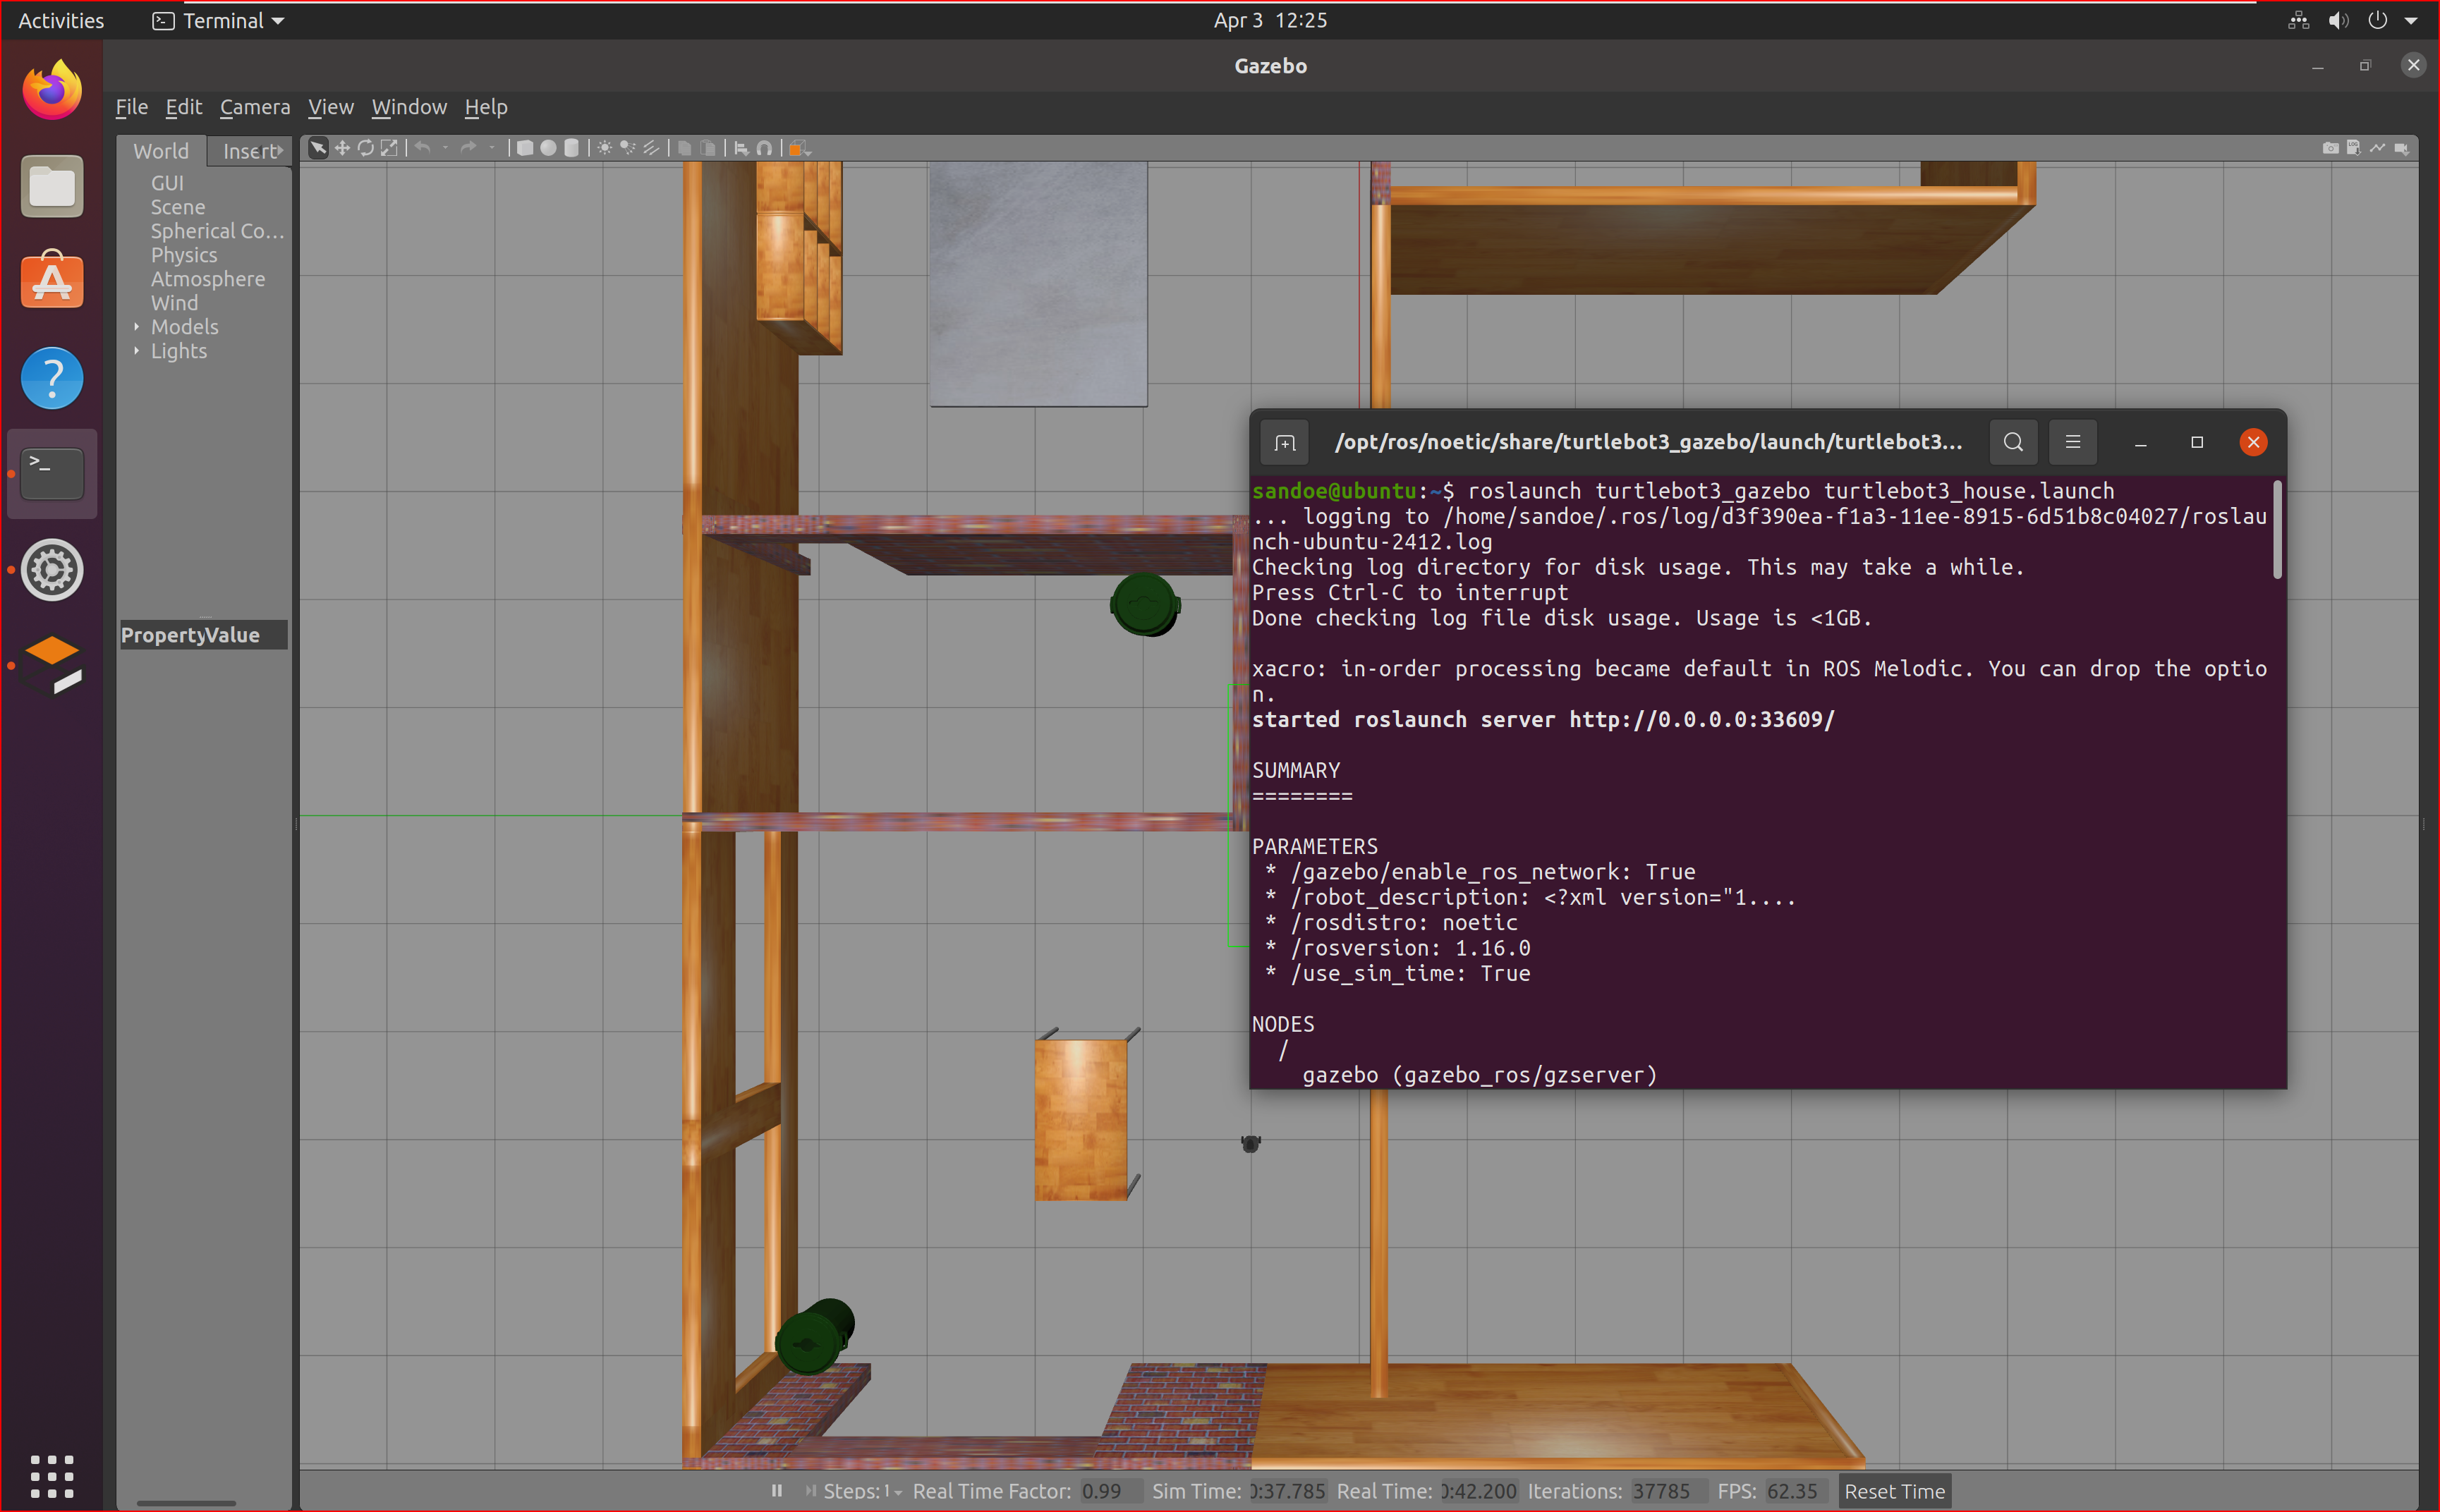
\includegraphics[width=\linewidth]{fig1.png}
		\caption{Simulation environment in Ubuntu (Fosscal), Gazebo V11 and Turtlebot3}
		\label{fig:fig1}
	\end{figure}
	The Turtlebot model is missing it's camera and therefore we need to terminate the session and navigate to following folder \texttt{catkin\_ws} for then be using the command \texttt{source devel/setup.bash}. We relaunch the simulation by following command:
	
	\noindent\texttt{roslaunch turtlebot3\_gazebo}\texttt{turtlebot3\_house.launch}.
	\\\\
	To verify that the camera and Lidar sensor is working then we are going to be running \texttt{rostopic list} followed up by \texttt{rostopic echo /scan} (Lidar) and \texttt{rostopic echo /camera/image\_raw}. By looking at the data stream then we can verify that the configuration is done and our environment running.
	\begin{figure}[!h]
		\centering
		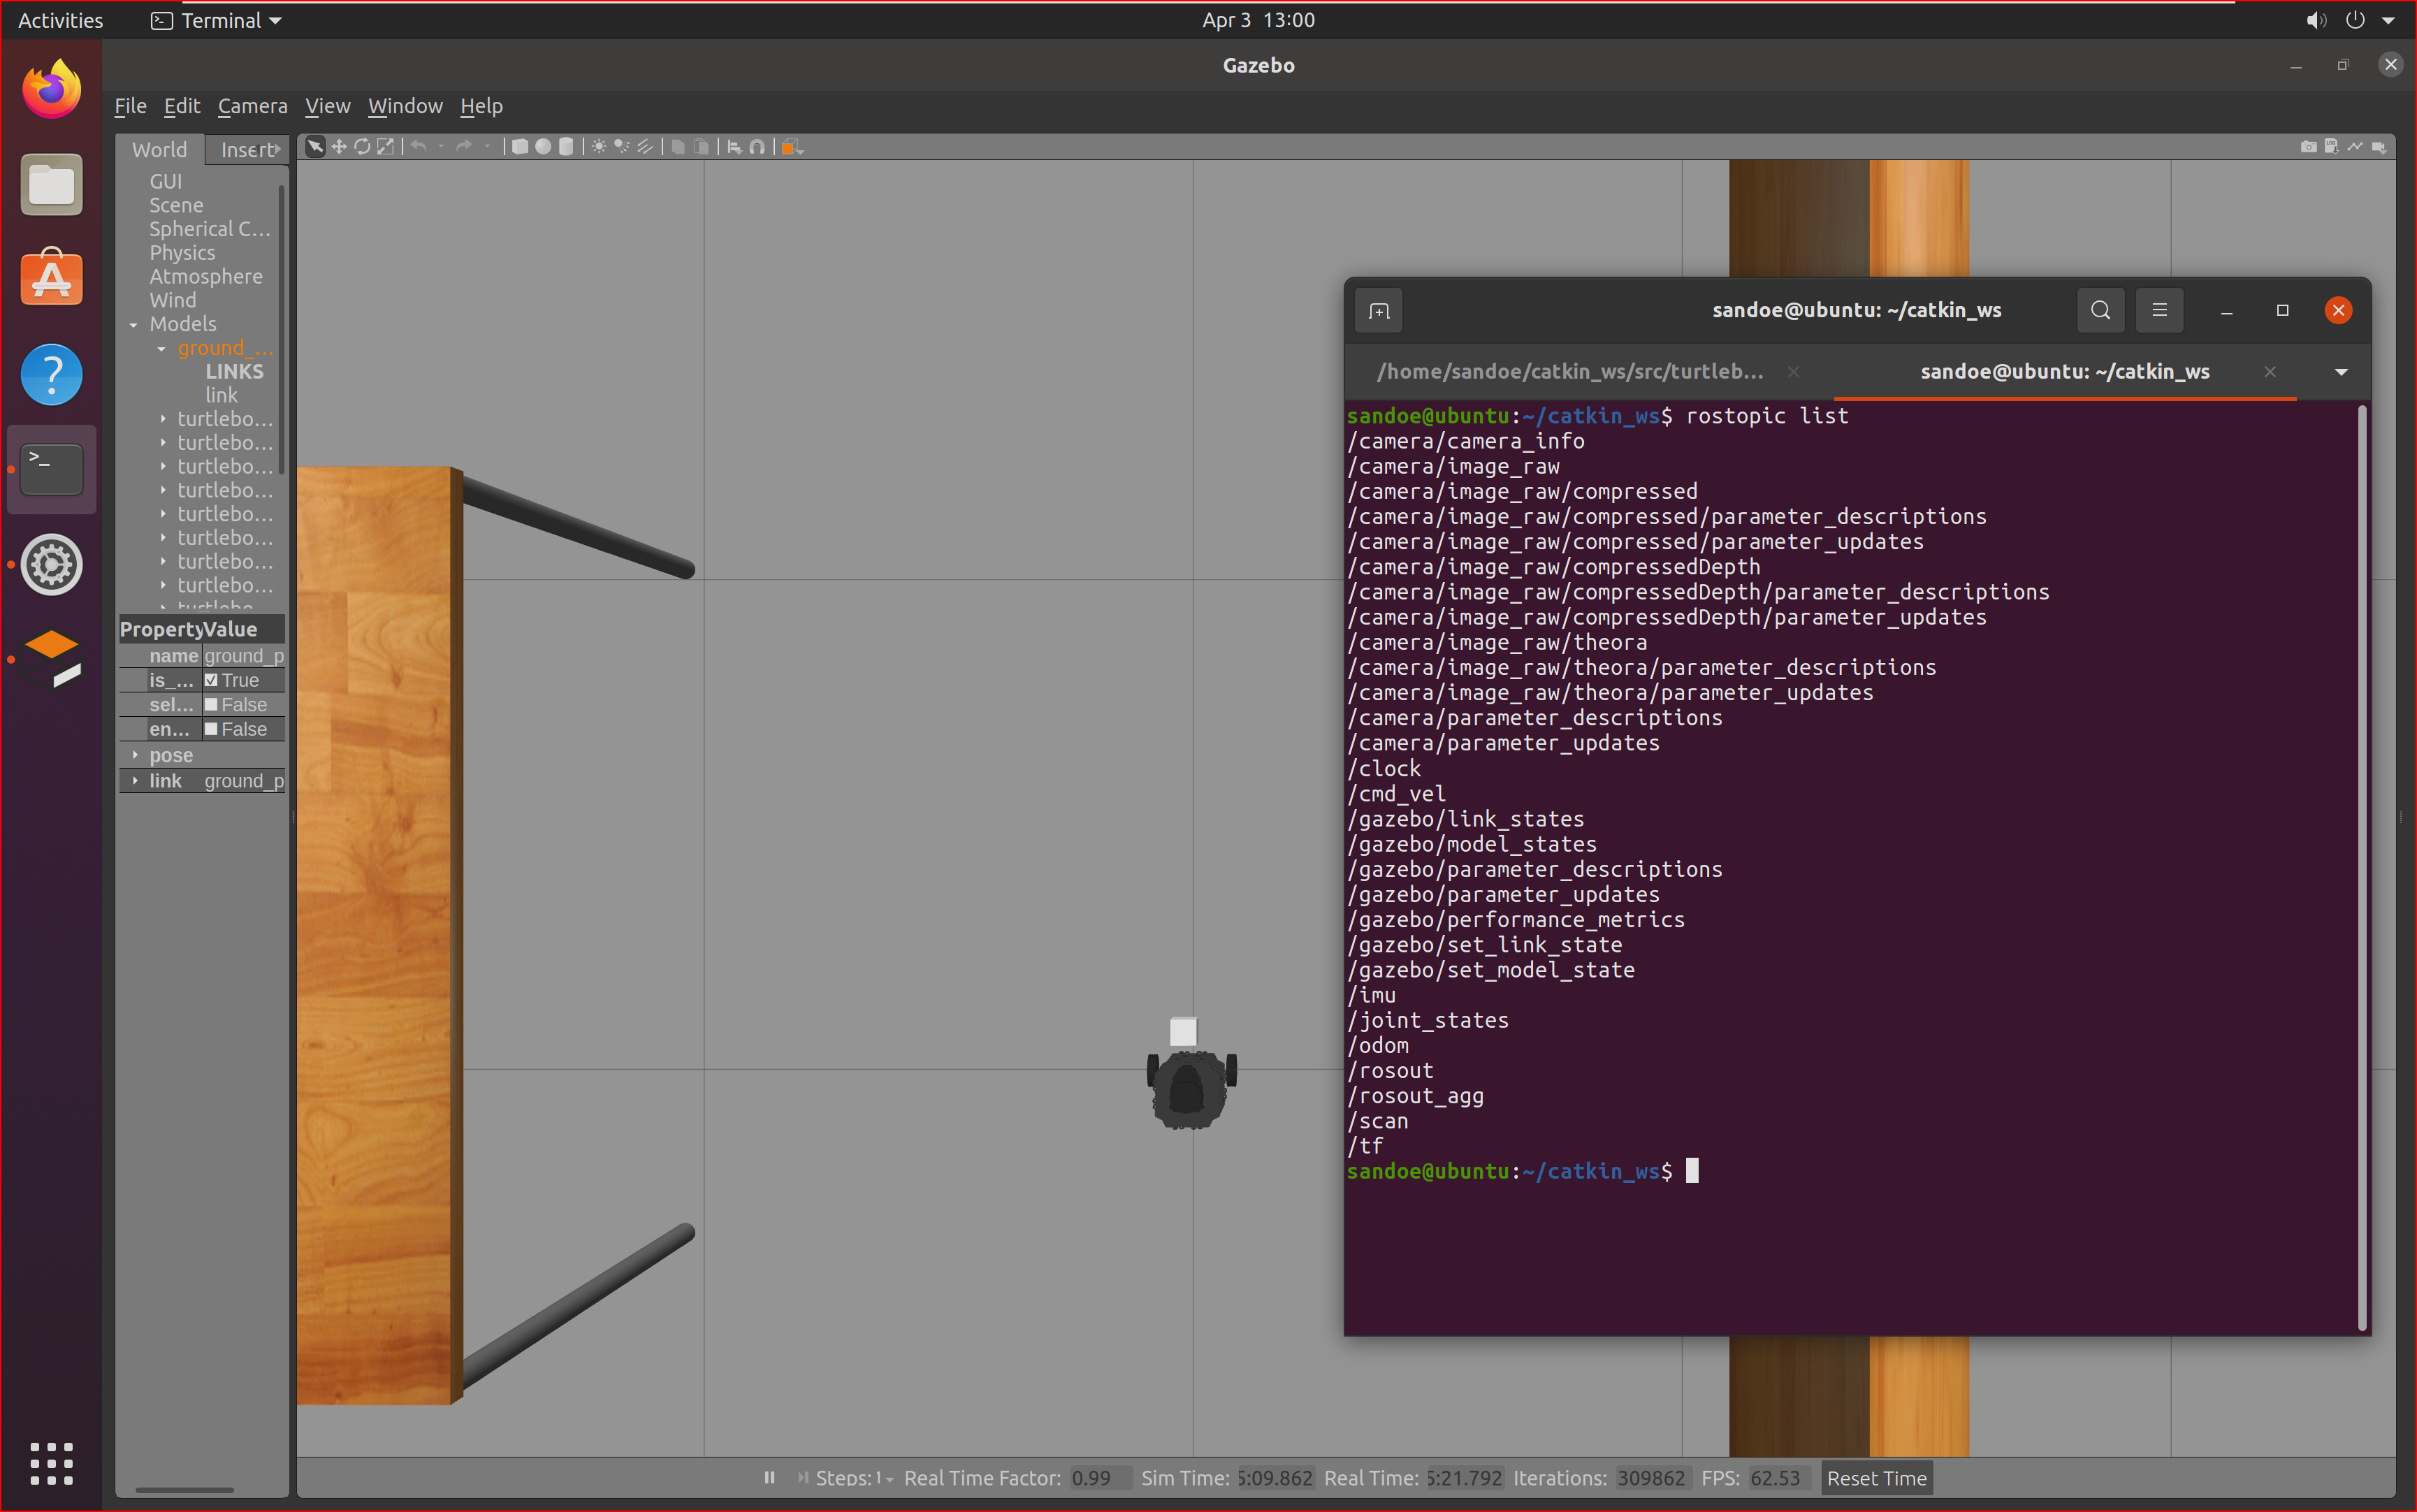
\includegraphics[width=\linewidth]{fig4.png}
		\caption{Showing rostopic list}
		\label{fig:fig4}
	\end{figure}
	\subsubsection{Simulation of Turtlebot behavior}
	
	\subsection{Physical Turtlebot}
	\subsubsection{Turtlebot and PC konfiguration}
	This section is for the physical Turtlebot and will describe how this task is going to be solved.
	\subsubsection{Connection to the TurtleBot3 from powershell}
	For making the connection to the turtlebot we are connecting to the WiFi 
	\begin{itemize}
		\item \textbf{ssid:} turtlebot
		\item \textbf{password:} turtlebot3
	\end{itemize}
	from powershell type:
	\begin{center}
		\textit{ssh ubuntu@192.168.72.251}, \textit{password: turtlebot}
	\end{center}
	\subsubsection{Starting ROS on turtlebot from powershell}
	from powershell type
	\begin{center}
		\textit{roscore}
	\end{center}
	\subsubsection{Connection to TurtleBot3 from Matlab}
	For setting the ros environment variable and setting the IP on the host (turtlebot):
	\begin{lstlisting}[style=Matlab-editor]
		setenv('ROS_MASTER_URI','http://192.168.72.251:11311')\end{lstlisting}
	For setting the IP on the local machine 
	\begin{lstlisting}
		setenv('ROS_IP','192.168.72.220')\end{lstlisting}
	The following command is closing existing connection to be ensure that when the user is connection the robot isn't connected to anyone else
	\begin{lstlisting}[style=Matlab-editor]
		rosshutdown();\end{lstlisting}
	This command will be doing the initialization of the connection between ROS and Matlab
	\begin{lstlisting}[style=Matlab-editor]
		rosinit('http://192.168.72.251:11311','NodeHost','192.168.72.220');\end{lstlisting} 
	\vspace{1cm}
	\noindent\textbf{Matlab script for init}
	\begin{lstlisting}[style=Matlab-editor]
		setenv('ROS_MASTER_URI','http://192.168.72.251:11311')
		setenv('ROS_IP','192.168.72.220')
		rosshutdown();
		rosinit('http://192.168.72.251:11311','NodeHost','192.168.72.220');\end{lstlisting}
\end{document}